\documentclass[a4paper, 11pt]{article}

\usepackage[utf8]{inputenc}
\usepackage[portuguese]{babel}
\usepackage[pdfborder={0 0 0}]{hyperref}
\usepackage{graphicx}
\usepackage{float}
\usepackage{a4wide}
\usepackage{indentfirst}
\usepackage{fancyhdr}
\usepackage{lastpage}
\usepackage{relsize}
\usepackage[intoc]{nomencl}
\makenomenclature
\renewcommand{\nomname}{Lista de Siglas e Acrónimos}

\title{Sistemas Operativos \\ [0.8em] \smaller{} Aurras: Processamento de Ficheiros de Áudio}
\author{João Freitas (A83782) \and Rui Fernandes (A89138)}
\date{Junho 2021}

\renewcommand\labelitemi{---}

\begin{document}

\begin{titlepage}
    \begin{center}
        \begin{minipage}{0.75\linewidth}
            \centering
            
\includegraphics[width=0.4\textwidth]{img/EEUM.png}\par\vspace{1cm}
            \vspace{1.5cm}
            \href{https://www.uminho.pt/PT}{\scshape\LARGE Universidade do Minho} \par
            \vspace{1cm}
            \href{https://www.di.uminho.pt/}{\scshape\Large Departamento de Informática} \par
            \vspace{1.5cm}
            \maketitle
        \end{minipage}
    \end{center}
    \vspace{2cm}
    \thispagestyle{empty}
    \clearpage
\end{titlepage}

\pagenumbering{roman}

\begin{abstract}
O presente relatório descreve o trabalho prático realizado no âmbito da disciplina de 
\href{http://miei.di.uminho.pt/plano_estudos.html#sistemas_operativos}{\emph {Sistemas 
Operativos}}, ao longo do segundo semestre do segundo ano do 
\href{http://miei.di.uminho.pt}{Mestrado Integrado em Engenharia Informática} da 
\href{https://www.uminho.pt}{Universidade do Minho}.

Com a realização deste trabalho prático, pretende-se implementar um serviço capaz de 
transformar ficheiros de áudio por aplicação de uma sequência de filtros, sendo que este 
deverá ser constituído por um servidor e por um cliente que deverão comunicar por \textit{pipes} 
com nome.

Neste documento descreve-se sucintamente a aplicação desenvolvida e discutem-se as decisões 
tomadas durante a realização do projeto.
\end{abstract}

\pagebreak

\tableofcontents
\listoffigures

\pagebreak

\pagenumbering{arabic}

\pagestyle{fancy}
\fancyhf{}

\rfoot{Página \thepage \hspace{1pt} de \pageref{LastPage}}

\renewcommand{\headrulewidth}{0pt}


\section{Introdução}
\label{sec:introducao}

No âmbito da Unidade Curricular de 
\href{http://miei.di.uminho.pt/plano_estudos.html#sistemas_operativos}{\emph {Sistemas 
Operativos}}, foi proposta a implementação de um serviço capaz de transformar ficheiros de 
áudio por aplicação de uma sequência de filtros, sendo que este deverá ser constituído por um 
servidor e um por cliente, que deverão comunicar por \textit{pipes} com nome. Tanto o cliente como 
o servidor apenas disponibilizam uma interface de linha de comandos.

\subsection*{Estrutura do Relatório}

O presente relatório encontra-se dividido em quatro partes distintas.

No capítulo \ref{sec:introducao}, Introdução, foi feito um enquadramento e uma breve 
contextualização do trabalho prático. 

De seguida, no capítulo \ref{sec:solucao}, Conceção da Solução, é feita uma descrição 
detalhada de todo o processo de desenvolvimento do trabalho prático até se obter a solução 
final.

No capítulo \ref{sec:resultados}, Análise de Resultados, são apresentados alguns testes 
realizados e os resultados obtidos.


Por fim, no capítulo \ref{sec:conclusao}, Conclusão, termina-se o relatório com uma síntese a 
análise
crítica do trabalho desenvolvido.

\pagebreak

\section{Conceção da Solução}
\label{sec:solucao}

\subsection{Implementação da Solução}

No desenvolvimento do presente trabalho prático, foi implementada uma arquitetura Cliente-Servidor 
com o intuito de distribuir processamento da informação entre o fornecedor do serviço -- 
servidor -- e os requerentes dos serviço -- clientes. Assim, os clientes enviam pedidos para o 
servidor e este, por sua vez, processa e envia os resultados dos respetivos pedidos. Note-se que os 
clientes e servidor comunicam através de \textit{pipes} com nome. 

Desta forma, um dos pontos centrais serão os mecanismos de comunicação entre processos (IPC), 
assim como a utilização das diferentes \textit{System Calls}.

Para controlo de erros foi também utilizada diversas vezes a função \texttt{perror} que imprime, 
se for o caso, uma mensagem de erro para o \texttt{stderr}.

Posto isto, importa também salientar que foram utilizados como ponto de partida a seguinte 
estrutura do código e a \texttt{Makefile} disponibilizados.

\

\begin{figure}[H]
    \centering
    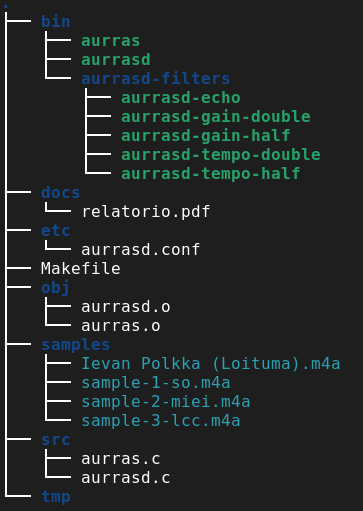
\includegraphics[width=.4\textwidth]{img/estrutura.png}
    \caption{Estrutura do código}
\end{figure}


\paragraph{Servidor\\}

No arranque do servidor, são criados dois \textit{pipes} com nome
que serão conhecidos por todos os clientes, um destinado aos pedidos dos clientes, e outro para o 
servidor enviar o seu estado atual. 

Ao receber um pedido de transformação de um ficheiro de áudio, o servidor primeiro verifica se o 
pedido foi enviado de forma correta e, nesse caso, verifica se todos os filtros solicitados se 
encontram disponíveis. Feitas as devidas verificações, cria-se um processo filho que será 
responsável por processar o pedido, \textit{i.e.}, por cada pedido recebido no servidor, é criado 
um processo filho que irá efetivamente tratar o pedido. Assim, este processo filho, recorrendo à 
\textit{system call} \texttt{execl} e a um correto redirecionamento de descritores de ficheiros, 
garante que os filtros são aplicados sequencialmente. Aqui, importa salientar que no caso do 
primeiro filtro, o \texttt{stdin} será o ficheiro de \textit{input} e, por oposição, no caso do 
último filtro, o \texttt{stdout} será o \textit{pipe} com nome criado pelo cliente para o efeito, 
sendo este responsável por guardar o ficheiro final. 
Por outro lado, ao receber um pedido sobre o seu estado atual, o servidor envia um sinal 
\texttt{SIGUSR1} a todos os processos filhos que, por sua vez, deverão enviar para o cliente, via 
\textit{pipe} com nome, informação relativa ao pedido que estão a processar. No caso do processo 
pai, este deverá enviar informação relativa à capacidade e disponibilidade dos filtros de 
áudio.

Por fim, ao receber um sinal \texttt{SIGTERM}, o servidor espera que o processamento atual dos 
ficheiros de áudio termine e, posteriormente, elimina os \textit{pipes} criados aquando do 
arranque.

\paragraph{Cliente\\}

Tal como referido anteriormente, o cliente apenas tem duas formas de interação com
o servidor -- efetuar um pedido de transformação de um ficheiro de áudio ou pedir a informação 
do estado do mesmo. 

Para implementar estas funcionalidades recorreu-se, em ambos os casos, ao uso de \textit{pipes} com 
nome. Assim, no caso da transformação de ficheiros de áudio, quando o cliente efetua um pedido, 
é criado um \textit{pipe} com nome, utilizando, para isso, o seu PID como identificador. Submetido 
o pedido, este espera a resposta do servidor e, posteriormente, cria o ficheiro final, eliminando, 
por fim, o \textit{pipe} criado.

Por outro lado, quando o cliente envia um pedido relativo ao estado do servidor, irá receber esta 
resposta através do \textit{pipe} com nome criado especificamente para este efeito. Após imprimir 
para o \texttt{stdout} esta informação, fecha o \textit{pipe} e termina a execução.

\vspace{1cm}

\subsection{Limitações da Solução Desenvolvida}

No seguimento da secção anterior, as limitações encontradas da solução implementada passam 
por:

\begin{itemize}
    \item Na eventualidade de o servidor não ter todos os filtros disponíveis, o pedido é 
descartado em vez de ficar em fila de espera até haver disponibilidade no servidor;
    \item Limitação quanto ao número máximo de pedidos a ser executados em simultâneo, assim 
como do número de filtros. 
\end{itemize}

\pagebreak

\subsection{Considerações Finais}

Apesar limitações anteriormente apresentadas, importa salientar que foram implementadas 
funcionalidades que oferecem grandes recursos ao servidor no que diz respeito a concorrência e 
desempenho, pelo que, de um modo geral, faz-se um balanço bastante positivo do trabalho 
desenvolvido. De facto:

\begin{itemize}
    \item O servidor inicia o tratamento dos pedidos de forma sequencial, suportando o 
processamento concorrente dos mesmos;
    \item Ao receber o sinal \texttt{SIGTERM}, o servidor termina de forma graciosa o seu 
funcionamento, isto é, termina
    os pedidos que em espera e só no fim termina o processo;
    \item Evita a criação de ficheiros temporários;
    \item O processamento de um pedido não é iniciado pelo servidor se não existirem instâncias 
disponíveis de todos os filtros necessários.
\end{itemize}

\pagebreak

\section{Análise de Resultados}
\label{sec:resultados}

\subsection*{Informação de Utilização}

\begin{figure}[H]
    \centering
    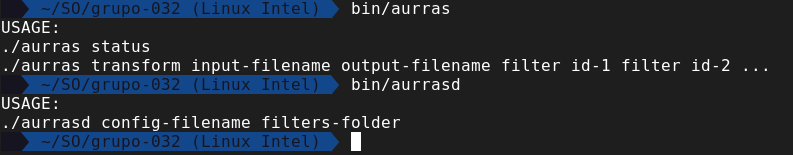
\includegraphics[width=.8\textwidth]{img/usage.png}
    \caption{Informação de utilização}
\end{figure}

\subsection*{Processamento de Ficheiros de Áudio}

\begin{figure}[H]
    \centering
    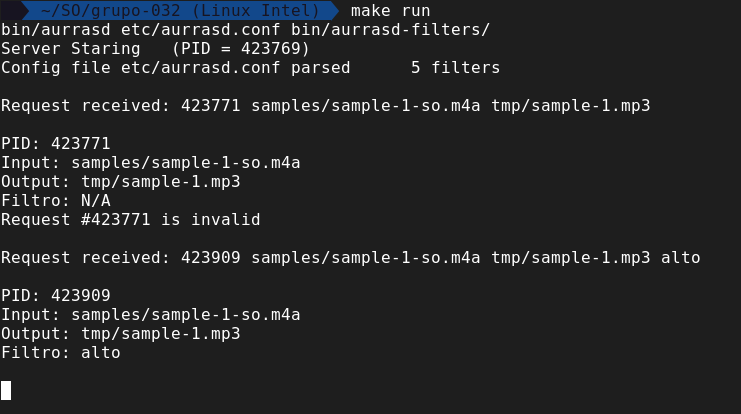
\includegraphics[width=.8\textwidth]{img/server.png}
    \caption{Processamento de ficheiros de áudio}
\end{figure}

\subsection*{Sinal \texttt{SIGTERM} \& Terminação do Servidor}

\begin{figure}[H]
    \centering
    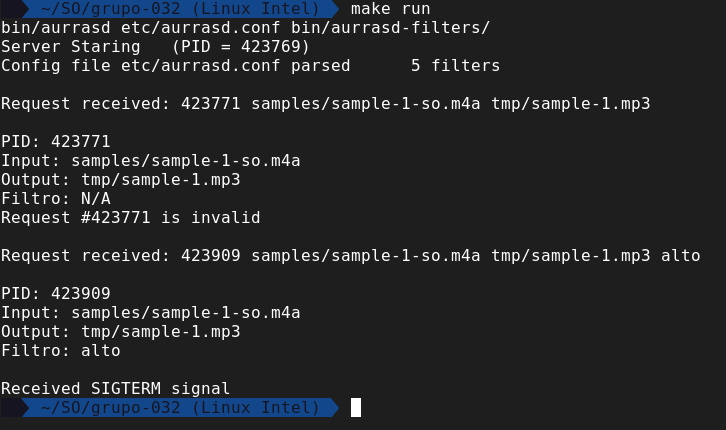
\includegraphics[width=.8\textwidth]{img/sigterm.png}
    \caption{Sinal \texttt{SIGTERM} \& terminação do servidor}
\end{figure}

\subsection*{Estado do Servidor}

\begin{figure}[H]
    \centering
    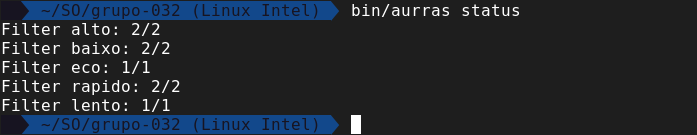
\includegraphics[width=.8\textwidth]{img/status_1.png}
    \caption{Estado do servidor}
\end{figure}

\begin{figure}[H]
    \centering
    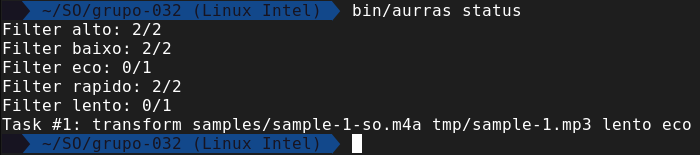
\includegraphics[width=.8\textwidth]{img/status_2.png}
    \caption{Estado do servidor}
\end{figure}

\pagebreak

\section{Conclusão}
\label{sec:conclusao}

Face ao problema apresentado e analisando criticamente a solução proposta concluímos que 
cumprimos as tarefas propostas, conseguindo atingir os objetivos definidos. De facto, foram 
implementadas todas as funcionalidades apresentadas. Assim, após a elaboração deste trabalho 
prático, pode-se afirmar que aprimoramos o nosso domínio sobre a linguagem de programação 
\texttt{C}, nomeadamente o uso das \textit{System Calls}, que foram a base do nosso trabalho.

No entanto, o grupo consegue reconhecer que, com uma melhor gestão do tempo, teria sido possível 
aprimorar as funcionalidades feitas até ao presente.

Como trabalho futuro, poderia ser implementado um histórico associado a um dado cliente e as 
tarefas executadas por esse mesmo cliente, entre outras. Neste sentido, importa salientar que a 
base de cliente e servidor implementada permite futura
escalabilidade.

\newpage

\nomenclature[01]{IPC}{\textit{Inter-process Communication}}
\nomenclature[02]{PID}{\textit{Process ID}}
\nomenclature[03]{\texttt{stderr}}{\textit{Standard Error}}
\nomenclature[04]{\texttt{stdin}}{\textit{Standard Input}}
\nomenclature[05]{\texttt{stdout}}{\textit{Standard Output}}

\printnomenclature

\end{document}
